%% Missed a few sections when Romy was born. (4.1, 4.2)
%% SEC 4.1
%%\section{Vector Spaces and Subspaces}
%% SEC 4.2
%%\section{Null Spaces, Column Spaces, and Linear Transformations}


% SEC 4.3
\setcounter{section}{2}
\section{Linearly Independent Sets; Bases}
\name[2in]


\begin{boxdef}
An indexed set of vectors $\B=\vectset[b]{1}{p}$ in $V$ is a \textbf{basis} for a subspace $H$ of $V$ if
\begin{enumerate}[(i)]
	\item $\B$ is a linearly independent set, and
	\item $H=\Span\vectset[b]{1}{p}$, i.e., the vectors $\vect{b}_1,\ldots,\vect{b}_p$ span $H$ (and no more than $H$).
\end{enumerate}
\end{boxdef}


\begin{exercise} % 4.3.1
	Determine if the set is linearly independent, if it spans $\R^3$, and if it is a basis for $\R^3$. Show work or explain your answer.
	$$ \left\{
	\begin{bmatrix}2\\2\\0\end{bmatrix},
	\begin{bmatrix}0\\2\\2\end{bmatrix},
	\begin{bmatrix}0\\2\\0\end{bmatrix}
	\right\} $$
	Circle all that apply:
	\begin{center}
	\shortstack{\textbf{Linearly Independent?} \\[1ex]
		\textbf{Yes \qquad No}} \hspace{5em}
	\shortstack{\textbf{\textbf{Spans} $\boldsymbol{\R^3}$?} \\[1ex]
		\textbf{Yes \qquad No}} \hspace{5em}
	\shortstack{\textbf{\textbf{Is a Basis for} $\boldsymbol{\R^3}$?} \\[1ex]
		\textbf{Yes \qquad No}}
	\end{center}
\end{exercise}
\vfill


\begin{exercise} % 4.3.5
	Determine if the set is linearly independent, if it spans $\R^3$, and if it is a basis for $\R^3$. Show work or explain your answer.
	$$ \left\{
	\begin{bmatrix}1\\-3\\0\end{bmatrix},
	\begin{bmatrix}-2\\3\\0\end{bmatrix},
	\begin{bmatrix}0\\0\\0\end{bmatrix},
	\begin{bmatrix}0\\-3\\5\end{bmatrix}
	\right\} $$
	Circle all that apply:
	\begin{center}
		\shortstack{\textbf{Linearly Independent?} \\[1ex]
			\textbf{Yes \qquad No}} \hspace{5em}
		\shortstack{\textbf{\textbf{Spans} $\boldsymbol{\R^3}$?} \\[1ex]
			\textbf{Yes \qquad No}} \hspace{5em}
		\shortstack{\textbf{\textbf{Is a Basis for} $\boldsymbol{\R^3}$?} \\[1ex]
			\textbf{Yes \qquad No}}
	\end{center}
\end{exercise}
\vfill


\newpage

\begin{boxme}
	To find a basis for $\Nul A$, write the general solution of $\Axz$ in parametric vector form. The vectors in the solution form a basis for $\Nul A$ (whenever $\Nul A \neq \{\vect{0}\}$)
\end{boxme}
\begin{boxthm}
	\textbf{Theorem 4.6.} \\
	The pivot columns of a matrix $A$ form a basis for $\Col A$.
\end{boxthm}

\begin{exercise} % 4.3.13
	Assume that $A$ is row equivalent to $B$.
	\begin{align*}
	A &= \begin{bmatrix} -2&4&-2&-4 \\ 2&-6&-6&1 \\ -3&8&5&-3 \end{bmatrix} &
	B &= \begin{bmatrix} 1&0&9&5 \\ 0&2&8&3 \\ 0&0&0&0 \end{bmatrix}
	\end{align*}
	\begin{multicols}{2}
		\begin{enumerate}[(a)]
			\item Find a basis for $\Nul A$.
			\item Find a basis for $\Col A$.
		\end{enumerate}
	\end{multicols}
\end{exercise}
\vfill


\begin{boxthm}
	\textbf{Theorem 4.5.}
	\textbf{The Spanning Set Theorem} \\
	Let $S=\vectsetvp$ be a set in $V$, and let $H=\Span\vectsetvp$.
	\begin{enumerate}[a.]
		\item If one of the vectors in $S$---say, $\vect{v}_k$---is a linear combination of the remaining vectors in $S$, then the set formed from $S$ by removing $\vect{v}_k$ still spans $H$.
		\item If $H\neq\{\vect{0}\}$, some subset of $S$ is a basis for $H$.
	\end{enumerate}
\end{boxthm}
\begin{exercise} % 4.3.19
	Let $\vect{v}_1 = \begin{bmatrix} 1\\2\\3 \end{bmatrix}$, $\vect{v}_2 = \begin{bmatrix} 3\\2\\1 \end{bmatrix}$, and $\vect{v}_3 = \begin{bmatrix} 4\\4\\4 \end{bmatrix}$. Note that $\vect{v}_1+\vect{v}_2=\vect{v}_3$. Find a basis for the subspace $H=\Span\{\vect{v}_1,\vect{v}_2,\vect{v}_3\}$.
\end{exercise}
\vspace{1in}


\newpage


% SEC 4.4
\section{Coordinate Systems}
\name

\begin{boxdef}
	Suppose $\B=\vectset[b]{1}{n}$ is a basis for $V$ and $\vect{x}$ is in $V$. The \textbf{coordinates of $\boldsymbol{\vect{x}}$ relative to the basis $\boldsymbol{\B}$} (or the $\boldsymbol{\B}$\textbf{-coordinates of} $\boldsymbol{\vect{x}}$) are the weights $c_1,\ldots,c_n$ such that $\vect{x} = c_1\vect{b}_1 + \cdots + c_n\vect{b}_n$.
	\begin{align*}
	\vectB &= \begin{bmatrix}[c]c_1 \\ \vdots \\ c_n\end{bmatrix}
	\end{align*}
	We call $\vectB$ the \textbf{coordinate vector of $\boldsymbol{\vect{x}}$ (relative to $\boldsymbol{\B}$)} or the \textbf{$\boldsymbol{\B}$-coordinate vector of $\boldsymbol{\vect{x}}$}.
\end{boxdef}


\begin{exercise} % 4.4.Custom (Graphical Interpretation)
	\begin{multicols}{2}
	The vectors $\vect{b}_1=\begin{bmatrix}2\\1\end{bmatrix}$, $\vect{b}_2=\begin{bmatrix}1\\3\end{bmatrix}$, and $\vect{x}=\begin{bmatrix}-4\\3\end{bmatrix}$ are shown in the figure. The vectors $\vect{b}_1$ and $\vect{b}_2$ provide a basis for $\R^2$, $\B=\{\vect{b}_1,\vect{b}_2\}$. This basis provides a new ``coordinate system'' as shown in the figure.
	
	Using the figure, find $\vectB = \begin{bmatrix}c_1 \\ c_2\end{bmatrix}$.
	
	\columnbreak
	
	\begin{center}
	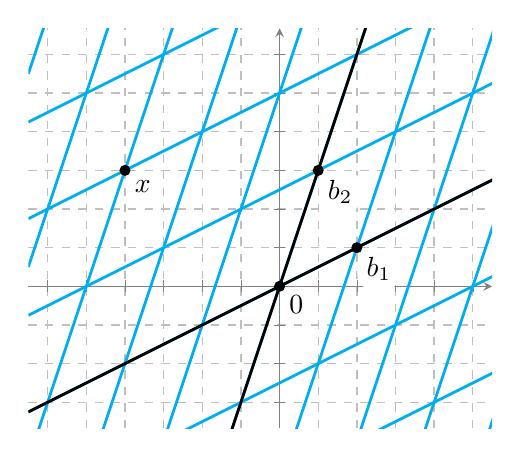
\begin{tikzpicture}[scale=1]
	% Set u and v
	\pgfmathsetmacro{\ux}{2}
	\pgfmathsetmacro{\uy}{1}
	\pgfmathsetmacro{\vx}{1}
	\pgfmathsetmacro{\vy}{3}
	\pgfmathsetmacro{\xcoor}{-4}
	\pgfmathsetmacro{\ycoor}{3}
	% Begin Axis
	\begin{axis}[axis x line=center, axis y line=middle,
	xmin=-6.5, xmax=5.5,
	ymin=-3.5, ymax=6.5,
	xtick={-6,...,5}, ytick={-3,...,7},
	xticklabels={,,}, yticklabels={,,},
	scale only axis, axis equal, height=2in,
	gray,
	grid=major, grid style={line width=.5pt, draw=gray!50, dashed}]
	% Plot alternate coordinate system
	\foreach \yi in {-10,...,10}{
		\addplot[-, cyan, line width=1pt, domain=-6.5:6.5] {(\uy/\ux)*(x-\yi*\vx)+\vy*\yi};
	}
	\foreach \xi in {-10,...,10}{
		\addplot[-, cyan, line width=1pt, domain=-6.5:6.5] {(\vy/\vx)*(x-\xi*\ux)+\uy*\xi};
	}
	\addplot[-, black, line width=1pt, domain=-6.5:6.5] {(\uy/\ux)*x};
	\addplot[-, black, line width=1pt, domain=-6.5:6.5] {(\vy/\vx)*x};
	% Plot vectors
	\fill[black] (0,0) circle (2pt) node[below right, fill=white, rounded corners=0.2cm] {$\vect{0}$};
	\fill[black] (\ux,\uy) circle (2pt) node[below right, fill=white, rounded corners=0.2cm] {$\vect{b}_1$};
	\fill[black] (\vx,\vy) circle (2pt) node[below right, fill=white, rounded corners=0.2cm] {$\vect{b}_2$};
	\fill[black] (\xcoor,\ycoor) circle (2pt) node[below right, fill=white, rounded corners=0.2cm] {$\vect{x}$};
	\end{axis}
	\end{tikzpicture}
	\end{center}
	\end{multicols}
\end{exercise}
\vspace{1in}


\begin{boxdef}
	For coordinates in $\R^n$, the \textbf{change-of-coordinates matrix} from $\B$ to the standard basis in $\R^n$, $$P_\B=\begin{bmatrix}\vect{b}_1&\cdots&\vect{b}_n\end{bmatrix},$$
	is used to transform $\vectB$ into $\vect{x}$ via the \textbf{change-of-coordinates equation}, $\vect{x}=P_\B\vectB$.
\end{boxdef}
\begin{exercise} % 4.4.7&9 Sort of
	Given $\B=\left\{ \begin{bmatrix}1\\-1\\-2\end{bmatrix}, \begin{bmatrix}-2\\3\\4\end{bmatrix}, \begin{bmatrix}1\\-1\\4\end{bmatrix} \right\}$ and $\vectB=\begin{bmatrix}-1\\1\\-3\end{bmatrix}$, answer the following.
	\begin{multicols}{2}
		\begin{enumerate}[(a)]
			\item Find the change-of-coordinates matrix, $P_\B$.
			\item Use $P_\B$ to find $\vect{x}$.
		\end{enumerate}
	\end{multicols}
\end{exercise}
\vfill


\newpage


\begin{boxdef}
	The \textbf{change-of-coordinates equation} is $\vect{x}=P_\B\vectB$. To find $\vectB$, you may solve the linear system $P_\B\vectB=\vect{x}$ or use the equation $\vectB=P_\B^{-1}\vect{x}$.
\end{boxdef}
\begin{exercise} % 4.4.5
	Find the coordinate vector $\vectB$ of $\vect{x}$ relative to the basis $\B=\{\vect{b}_1,\vect{b}_2\}$.
	\begin{align*}
	\vect{b}_1 &= \begin{bmatrix}2\\3\end{bmatrix} &
	\vect{b}_2 &= \begin{bmatrix}-5\\-1\end{bmatrix} &
	\vect{x} &= \begin{bmatrix}3\\-2\end{bmatrix}
	%& \vectB &=\begin{bmatrix}-1\\-1\end{bmatrix}
	\end{align*}
%% \R^3 Version might be too long:
%	Find the coordinate vector $\vectB$ of $\vect{x}$ relative to the basis $\B=\{\vect{b}_1,\vect{b}_2,\vect{b}_3\}$.
%	\begin{align*}
%	\vect{b}_1 &= \begin{bmatrix}1\\-1\\-3\end{bmatrix} &
%	\vect{b}_2 &= \begin{bmatrix}4\\-3\\-12\end{bmatrix} &
%	\vect{b}_3 &= \begin{bmatrix}2\\-2\\10\end{bmatrix} &
%	\vect{x} &= \begin{bmatrix}-5\\4\\-1\end{bmatrix}
%	%& \vectB &=\begin{bmatrix}1\\-1\\-1\end{bmatrix}
%	\end{align*}
\end{exercise}
\vfill


\begin{boxthm}
	\textbf{Theorem 4.8.} \\
	Let $\B=\vectset[b]{1}{n}$ be a basis for a vector space $V$. Then the coordinate mapping $\vect{x}\mapsto\vectB$ is a one-to-one linear transformation from $V$ onto $\R^n$.
\end{boxthm}
\vspace{-1em}
\begin{boxme}
	If a vector space $V$ has a basis of $n$ vectors, Theorem 4.8 says that vectors from $V$ will ``act like'' vectors in $\R^n$ under linear transformations. This is particularly useful for vector spaces whose standard basis is something other than the usual coordinate vectors we're used to. For example, the standard basis for, $\Poly_n$, the vector space of polynomials of degree at most $n$, is $\B=\{1,t,t^2,...,t^n\}$. Theorem 4.8 allows us to rewrite polynomials in $\Poly_n$ using coordinates in $\R^{n+1}$ instead (since $\B$ contains $n+1$ vectors).
\end{boxme}
\begin{exercise} % 4.4.13
	The set $\B=\{ 1-t^2, -2t+t^2, 1+t-t^2 \}$ is a basis for $\Poly_2$. Find $\vectB[p]$, the coordinate vector of $\vect{p}(t)=1-7t+2t^2$ relative to $\B$. \\

	Hint: You are trying to find $c_1$, $c_2$, and $c_3$, so that
	\begin{align*}
	c_1(1-t^2)+c_2(-2t+t^2)+c_3(1+t-t^2) &= 1-7t+2t^2. \\
	\text{Reordering terms gives:}\quad
	(c_1+c_3) + (-2c_2+c_3)t + (-c_1+c_2-c_3)t^2 &= 1-7t+2t^2.
	\end{align*}
	Noting that the coefficients on the left and right hand side have to match, use this equation to come up with a system of 3 linear equations in the unknowns $c_1$, $c_2$, and $c_3$. Solving the system will give you $\vectB[p]$.
\end{exercise}
\vfill


\newpage


% SEC 4.5
\section{The Dimension of a Vector Space}
\name[2in]


\begin{boxthm}
	\textbf{Theorem 4.10.} \\
	If a vector space $V$ has a basis of $n$ vectors, then very basis for $V$ must consist of exactly $n$ vectors.
\end{boxthm}
\vspace{-1em}
\begin{boxdef}
	The \textbf{dimension} of a vector space $V$, denoted $\dim V$, is the number of vectors in a basis for $V$.
\end{boxdef}

\begin{exercise} % 4.5.1 Custom
	$$\left\{ \begin{bmatrix}[c] 4s - 2t \\ -3s + t \\ 3t \end{bmatrix} : s,t \text{ in } \R \right\}$$
	\begin{enumerate}[(a)]
		\item Find a basis for the subspace given above. \\
		(Hint: First write the subspace as a linear combination of vectors with $s$ and $t$ as parameters.)
		\vfill
		\item State the dimension of the subspace.
		\vspace{2em}
	\end{enumerate}
\end{exercise}


\begin{boxme}
	The dimension of $\Nul A$ is the number of free variables in the equation $\Axz$. \\
	The dimension of $\Col A$ is the number of pivot columns in $A$.
\end{boxme}


\begin{exercise} % 4.5.13 & 15
	Determine the dimensions of the null space and column space for each matrix below.
	\begin{multicols}{2}
	\begin{enumerate}[(a)]
		\item $$A=\begin{bmatrix}1&-5&-5&3&-6\\0&1&7&-2&2\\0&0&0&-6&-9\\0&0&0&0&1\end{bmatrix}$$
		\vspace{2em}
		
		$\boldsymbol{\dim\Nul A=}$ \\[1em]
		$\boldsymbol{\dim\Col A=}$
		
		\columnbreak
		
		\item $$B=\begin{bmatrix}1&0&2&6&5&-3\\0&0&1&-2&4&6\end{bmatrix}$$
		\vspace{2em}
		
		$\boldsymbol{\dim\Nul B=}$ \\[1em]
		$\boldsymbol{\dim\Col B=}$
	\end{enumerate}
	\end{multicols}
\end{exercise}
\vspace{1in}


\newpage


%\begin{exercise} % 4.5.11
%	Find the dimension of the subspace spanned by the given vectors.
%	$$ \begin{bmatrix}1\\0\\-4\end{bmatrix}, 
%	\begin{bmatrix}1\\1\\-3\end{bmatrix}, 
%	\begin{bmatrix}1\\4\\0\end{bmatrix}, 
%	\begin{bmatrix}-1\\-3\\1\end{bmatrix}$$
%\end{exercise}
%\vfill

\begin{boxthm}
	\textbf{Theorem 4.9.} \\
	If a vector space $V$ has a basis $\B=\vectset[b]{1}{n}$, then any set in $V$ containing more than $n$ vectors must be linearly dependent.
\end{boxthm}
\vspace{-1em}
\begin{boxthm}
	\textbf{Theorem 4.12.}
	\textbf{The Basis Theorem} \\
	Let $V$ be a $p$-dimensional vector space, $p\geq 1$. Any linearly independent set of vectors of exactly $p$ elements in $V$ is automatically a basis for $V$. Any set of exactly $p$ elements that spans $V$ is automatically a basis for $V$.
\end{boxthm}


\begin{exercise} % 4.5.Custom
	Use the above theorems to answer the questions here.
	\begin{multicols}{2}
		\begin{enumerate}[(a)]
			\item The set of vectors below span $\R^5$.
			$$\left\{
			\begin{bmatrix}1\\2\\1\\0\\1\end{bmatrix},
			\begin{bmatrix}1\\0\\1\\1\\1\end{bmatrix},
			\begin{bmatrix}1\\2\\1\\3\\1\end{bmatrix},
			\begin{bmatrix}1\\2\\3\\1\\1\end{bmatrix},
			\begin{bmatrix}1\\0\\0\\0\\0\end{bmatrix},
			\begin{bmatrix}0\\0\\0\\0\\1\end{bmatrix}
			\right\}$$
			Is this set a basis for $\R^5$? Explain.
			
			\columnbreak
			\item The polynomials in the set below are linearly independent.
			$$ \{1, 2t , -2+4t^2 ,  -12t+8t^3 \} $$
			Is this set a basis for $\Poly_3$? Explain
		\end{enumerate}
	\end{multicols}
\end{exercise}
\vspace{1in}


\begin{exercise} % 4.5.6
	This exercise is similar to the first one, but there is an extra step involved.
	$$\left\{ \begin{bmatrix}[c] 3a+6b-1c \\ 6a-2b-2c \\ -6a+5b+2c \\ -3a+b+c \end{bmatrix} : a,b,c \text{ in } \R \right\}$$
	\begin{enumerate}[(a)]
		\item Find a basis for the subspace given above. \\
		(Hint: Remember that basis vectors must span the space and be \emph{linearly independent}!)
		\vfill
		\item State the dimension of the subspace.
		\vspace{2em}
	\end{enumerate}
\end{exercise}


\newpage


% SEC 4.6
\section{Rank}
\name

\begin{boxdef}
	The \textbf{rank} of $A$ is the dimension of the column space of $A$.
\end{boxdef}

\begin{exercise} % 4.6.Custom
	\begin{enumerate}[(a)]
		\item Given the matrix $A$ below, determine the rank of $A$.\\
		$ A = \begin{bmatrix} 1&-3&3&-2 \\ -3&7&-1&2 \\ 0&1&-4&3 \end{bmatrix} $
		\vfill
		\item The rank of $A$ can be described in terms of the pivot positions of $A$. Write a sentence explaining this relationship.
		\vspace{.75in}
	\end{enumerate}
\end{exercise}


\begin{boxdef}
	Rows of a matrix $A$ can be viewed as vectors. If $A=\begin{bmatrix}3&0&-2\\0&4&2\end{bmatrix}$, the row vectors are $\begin{bmatrix}3\\0\\-2\end{bmatrix}$ and $\begin{bmatrix}0\\4\\2\end{bmatrix}$.
	
	The \textbf{Row Space} of $A$, denoted $\Row A$, is the set of all linear combinations of the row vectors.
\end{boxdef}
\vspace{-1em}
\begin{boxthm}
	\textbf{Theorem 4.13.} \\
	If two matrices $A$ and $B$ are row equivalent, then their row spaces are the same. If $B$ is in echelon form, the nonzero rows of $B$ form a basis for the row space of $A$ as well as for that of $B$.
\end{boxthm}

\begin{exercise} % 4.6.3 - Just row space
	The given matrices $A$ and $B$ below are row equivalent.
	\begin{align*}
	A &= \begin{bmatrix}2&-3&6&2&5\\-2&3&-3&-3&-4\\4&-6&9&5&9\\-2&3&3&-4&1\end{bmatrix} &
	B &= \begin{bmatrix}2&-3&6&2&5\\0&0&3&-1&1\\0&0&0&1&3\\0&0&0&0&0\end{bmatrix}
	\end{align*}
	\begin{enumerate}[(a)]
		\item Determine a basis for $\Row A$.
		\vfill
		\item Are the rows of $A$ linearly independent? Explain? \\
		(Hint: compare the number of rows of $A$ and $\dim\Row A$.)
		\vspace{.5in}
	\end{enumerate}
\end{exercise}


\newpage


\begin{boxthm}
	\textbf{Theorem 4.14.}
	\textbf{The Rank Theorem} \\
	The dimension of the column space and the row space of an $m\times n$ matrix $A$ are equal. This common dimension, the rank of $A$, also equals the number of pivot positions in $A$ and satisfies the equation
	\vspace{-1em}
	$$ \rank A + \dim\Nul A = n. $$
\end{boxthm}

\begin{exercise} % 4.6.8
	Suppose a $7\times 9$ matrix $A$ has 5 pivots.
	\begin{multicols}{2}
		\begin{enumerate}[(a)]
			\item What is $\rank A$? How do you know?
			\item What is $\dim\Nul A$? Explain or show work.
		\end{enumerate}
	\end{multicols}
\end{exercise}
\vspace{1.5in}


\begin{exercise} % 4.6.2
	Assume that $A$ and $B$ are row equivalent.
	\begin{align*}
	A &= \begin{bmatrix}1&-3&-2&5&-5\\2&-2&-7&13&0\\-3&9&12&-21&-9\\-2&6&0&-6&0\end{bmatrix} &
	B &= \begin{bmatrix}1&-3&-2&5&-5\\0&0&1&-1&-4\\0&0&0&0&-2\\0&0&0&0&0\end{bmatrix}
	\end{align*}
	\begin{enumerate}[(a)]
		\item Determine $\rank A$ and $\dim\Nul A$.
		\begin{align*}
		\boldsymbol{\rank A} &=		& \boldsymbol{\dim\Nul A} &=
		\end{align*}
		\item Find a basis for each of the following 3 subspaces.
			\begin{multicols}{2}
				\begin{enumerate}[(i)]
					\item $\Col A$ \vspace{1in}
					\item $\Row A$
					
					\columnbreak
					\item $\Nul A$ % BONUS problem
				\end{enumerate}
			\end{multicols}
	\end{enumerate}
	
	
% Solution:
%A basis for $\Col A$ is
%$\left\{
%\begin{bmatrix}1\\2\\-3\\-2\end{bmatrix},
%\begin{bmatrix}-2\\-7\\12\\0\end{bmatrix},
%\begin{bmatrix}-5\\0\\-9\\0\end{bmatrix}
%\right\}$.
%
%A basis for $\Row A$ is
%$\left\{
%\begin{bmatrix}1\\-3\\-2\\5\\-5\end{bmatrix},
%\begin{bmatrix}0\\0\\1\\-1\\-4\end{bmatrix},
%\begin{bmatrix}0\\0\\0\\0\\-2\end{bmatrix}
%\right\}$.
%
%A basis for $\Nul A$ is
%$\left\{
%\begin{bmatrix}3\\1\\0\\0\\0\end{bmatrix},
%\begin{bmatrix}-3\\0\\1\\1\\0\end{bmatrix}
%\right\}$.
\end{exercise}
\vspace{1in}


\newpage


% SEC 4.7
\section{Change of Basis}
\name

\begin{boxdef}
	Recall the following from section 4.4:
	
	For coordinates in $\R^n$, the \textbf{change-of-coordinates matrix} from $\B$ to the standard basis, $\E$, is the matrix $P_\B=\CoC{\B}{\E}=\begin{bmatrix}\vect{b}_1&\cdots&\vect{b}_n\end{bmatrix}.$
	$P_\B$ is used to transform $\vectB$ into $\vect{x}$ via the \textbf{change-of-coordinates equation}, $\vect{x}=P_\B\vectB$. To find $\vectB$, solve the linear system $P_\B\vectB=\vect{x}$.
\end{boxdef}

\begin{exercise} % 4.4.5 (REVIEW)
% \R^3 Version might be too long:
	Find the coordinate vector $\vectB$ of $\vect{x}$ relative to the basis $\B=\{\vect{b}_1,\vect{b}_2,\vect{b}_3\}$.
	\begin{align*}
	\vect{b}_1 &= \begin{bmatrix}1\\-1\\-3\end{bmatrix} &
	\vect{b}_2 &= \begin{bmatrix}4\\-3\\-12\end{bmatrix} &
	\vect{b}_3 &= \begin{bmatrix}2\\-2\\10\end{bmatrix} &
	\vect{x} &= \begin{bmatrix}-5\\4\\-1\end{bmatrix}
	%& \vectB &=\begin{bmatrix}1\\-1\\-1\end{bmatrix}
	\end{align*}
\end{exercise}
\vfill


\begin{boxdef}
	In 4.4, the matrix $P_\B=\CoC{\B}{\E}$ was used to translate $\B$-coordinate vectors into vectors written in the standard basis. In a similar way, we can translate between any two bases $\B$ and $\C$ using the matrix $\CoC{\B}{\C}$ described in Theorem 4.15.
\end{boxdef}
\vspace{-1em}
\begin{boxthm}
	\textbf{Theorem 4.15.} 
	(\textbf{Change-of-Coordinates Matrix from $\boldsymbol{\B}$ to $\boldsymbol{\C}$}) \\
	Let $\B=\vectset[b]{1}{n}$ and $\C=\vectset[c]{1}{n}$ be bases of a vector space $V$. Then there is a unique $n\times n$ matrix $\CoC{\B}{\C}$ such that
	$$ \vectC = \CoC{\B}{\C}\vectB. $$
	The columns of $\CoC{\B}{\C}$ are the $\C$-coordinate vectors of the vectors in the basis $\B$. That is,
	$$ \CoC{\B}{\C} = \begin{bmatrix}\vectC[b_1]&\vectC[b_2]&\cdots&\vectC[b_3]\end{bmatrix}.$$
\end{boxthm}


\begin{exercise} % 4.7.2
	Let $\B=\{\vect{b}_1,\vect{b}_2\}$ and $\C=\{\vect{c}_1,\vect{c}_2\}$ be bases for a vector space $V$, and suppose $\vect{b}_1=-\vect{c}_1+4\vect{c}_2$ and $\vect{b}_2=5\vect{c}_1-3\vect{c}_2$.
	\begin{multicols}{2}
		\begin{enumerate}[(a)]
			\item Find the change-of-coordinates matrix from $\B$ to $\C$.
			\item Find $\vectC[x]$ for $\vect{x}=5\vect{b}_1+3\vect{b}_2$.
		\end{enumerate}
	\end{multicols}
\end{exercise}
\vfill


\newpage

\begin{boxme}
	If two bases for $\R^n$ are explicitly given, $\B=\vectset[b]{1}{n}$ and $\C=\vectset[c]{1}{n}$, you may find $\CoC{\B}{\C}$ via row reduction:
	$$\begin{bmatrix}\vect{c}_1&\cdots&\vect{c}_n&\vect{b}_1&\cdots&\vect{b}_n\end{bmatrix} \xrightarrow{\text{RREF}} \begin{bmatrix}I_n&\CoC{\B}{\C}\end{bmatrix}$$
	You may also use the formula $\CoC{\B}{\C}=(P_\C)^{-1}P_\B$.
	
	If you know $\CoC{\B}{\C}$, the inverse gives you the change-of-coordinates matrix from $\C$ to $\B$: $\CoC{\C}{\B} = \left(\CoC{\B}{\C}\right)^{-1}$.
\end{boxme}


\begin{exercise} % 4.7.7
	Let $\B=\left\{ \begin{bmatrix}7\\5\end{bmatrix},\begin{bmatrix}-3\\-1\end{bmatrix} \right\}$ and $\C=\left\{ \begin{bmatrix}1\\-5\end{bmatrix},\begin{bmatrix}-2\\2\end{bmatrix} \right\}$ be two bases for $\R^2$.
	\begin{multicols}{2}
		\begin{enumerate}[(a)]
			\item Find $\CoC{\B}{\C}$.
			\item Find $\CoC{\C}{\B}$.
		\end{enumerate}
	\end{multicols}
\end{exercise}
\vfill


\begin{exercise} % 4.7.13
	In $\Poly_1$, find the change-of-coordinates matrix from the basis $\B=\{ 1-2t , 3-5t \}$ to the standard basis $\C=\{1,t\}$. Then find the $\B$-coordinate vector for $5-8t$.
	\begin{multicols}{2}
		\begin{enumerate}[(a)]
			\item Find $\CoC{\B}{\C}$.
			\item Find the $\B$-coordinate vector for $5-8t$.
		\end{enumerate}
	\end{multicols}
\end{exercise}
\vfill


%% SEC 4.9 - No In-class work
%\setcounter{section}{8}
%\section{Applications to Markov Chains}


\newpage
